\chapter{Anhang}
\label{a:append}

\begin{figure}[h]
	\centering
	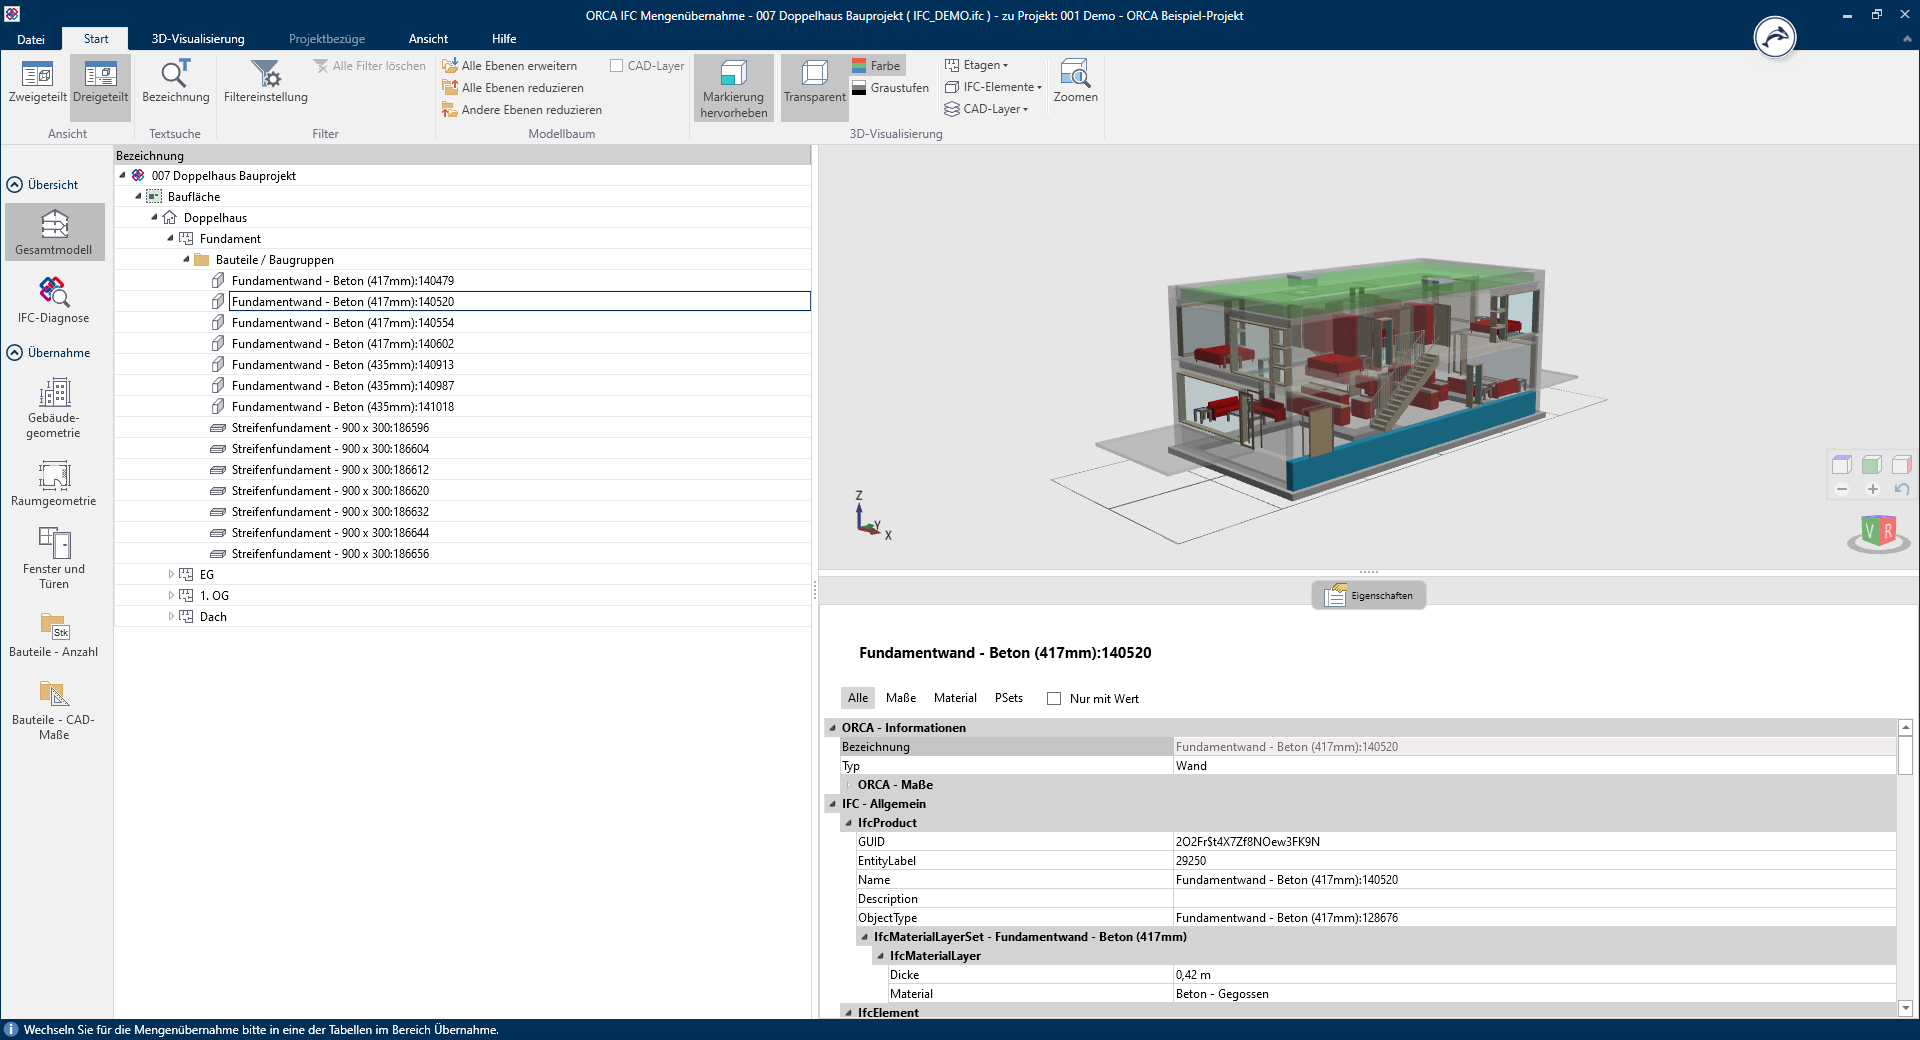
\includegraphics[width=1\linewidth]{ifc-manager}
	\caption[IFC Manager]{Oberfläche des \ac{ifc} Manager}
	\label{fig:ifc-manager}
\end{figure}

\begin{figure}[h]
	\centering
	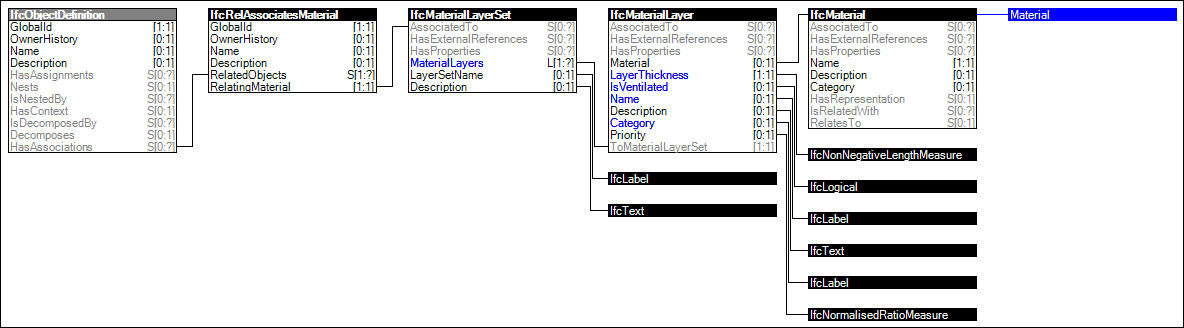
\includegraphics[width=1\linewidth]{material-layer-set}
	\caption[IfcMaterialLayerSet]{Material Layer Set Association}
	\label{fig:layer-set}
\end{figure}

\begin{figure}[h]
	\centering
	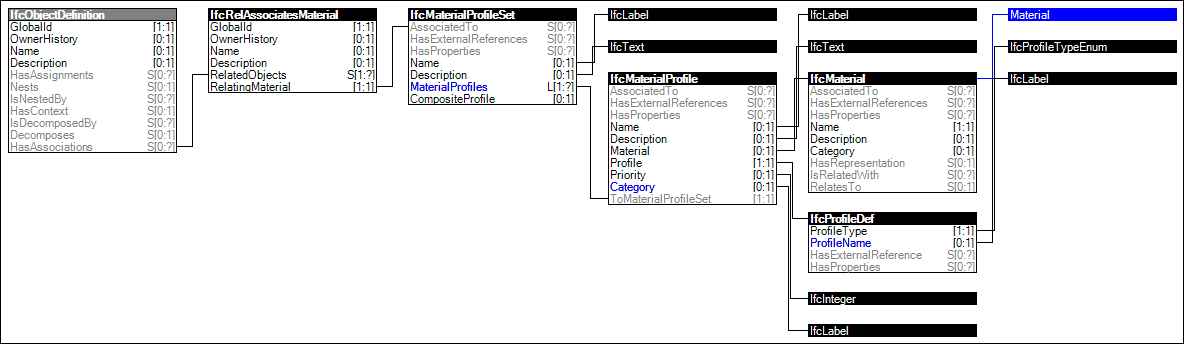
\includegraphics[width=1\linewidth]{material-profile-set}
	\caption[IfcMaterialProfileSet]{Material Profile Set Association}
	\label{fig:profile-set}
\end{figure}

\begin{figure}[h]
	\centering
	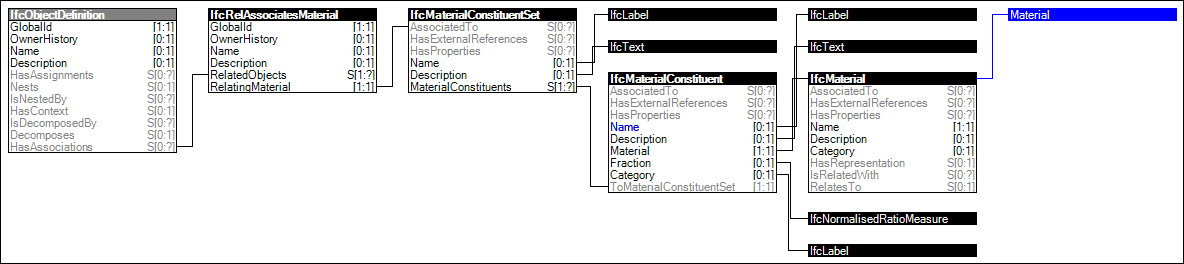
\includegraphics[width=1\linewidth]{material-constituent-set}
	\caption[IfcMaterialConsituentSet]{Material Constituent Set Association}
	\label{fig:constituent-set}
\end{figure}

\begin{figure}[h]
	\centering
	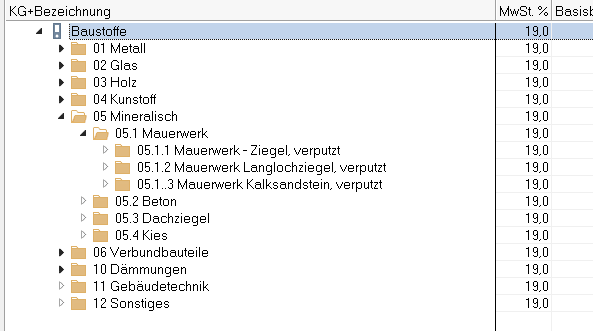
\includegraphics[width=1\linewidth]{cost-structure-example}
	\caption[CostStructure]{Beispiel einer Kostengliederung in der ORCA AVA}
	\label{fig:cost-structure}
\end{figure}

\begin{figure}[h]
	\centering
	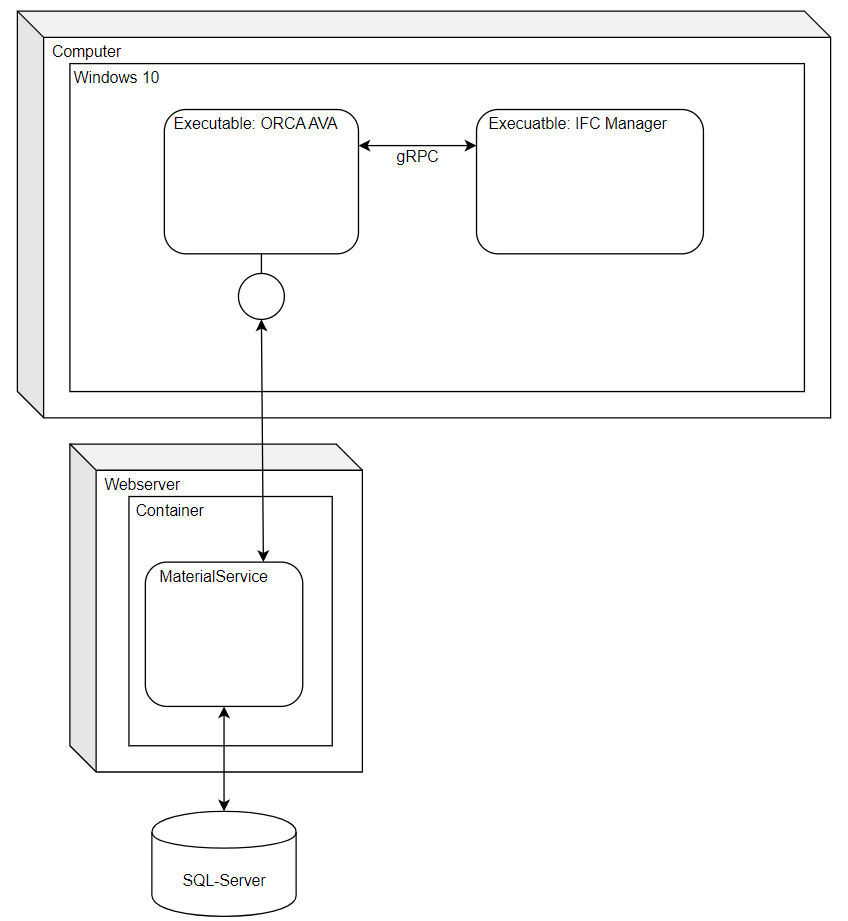
\includegraphics[width=1\linewidth]{verteilungsdiagramm}
	\caption[Verteilungsdiagramm]{Verteilungsdiagramm der Architektur}
	\label{fig:distribution-diagramm}
\end{figure}

\begin{figure}[h]
	\centering
	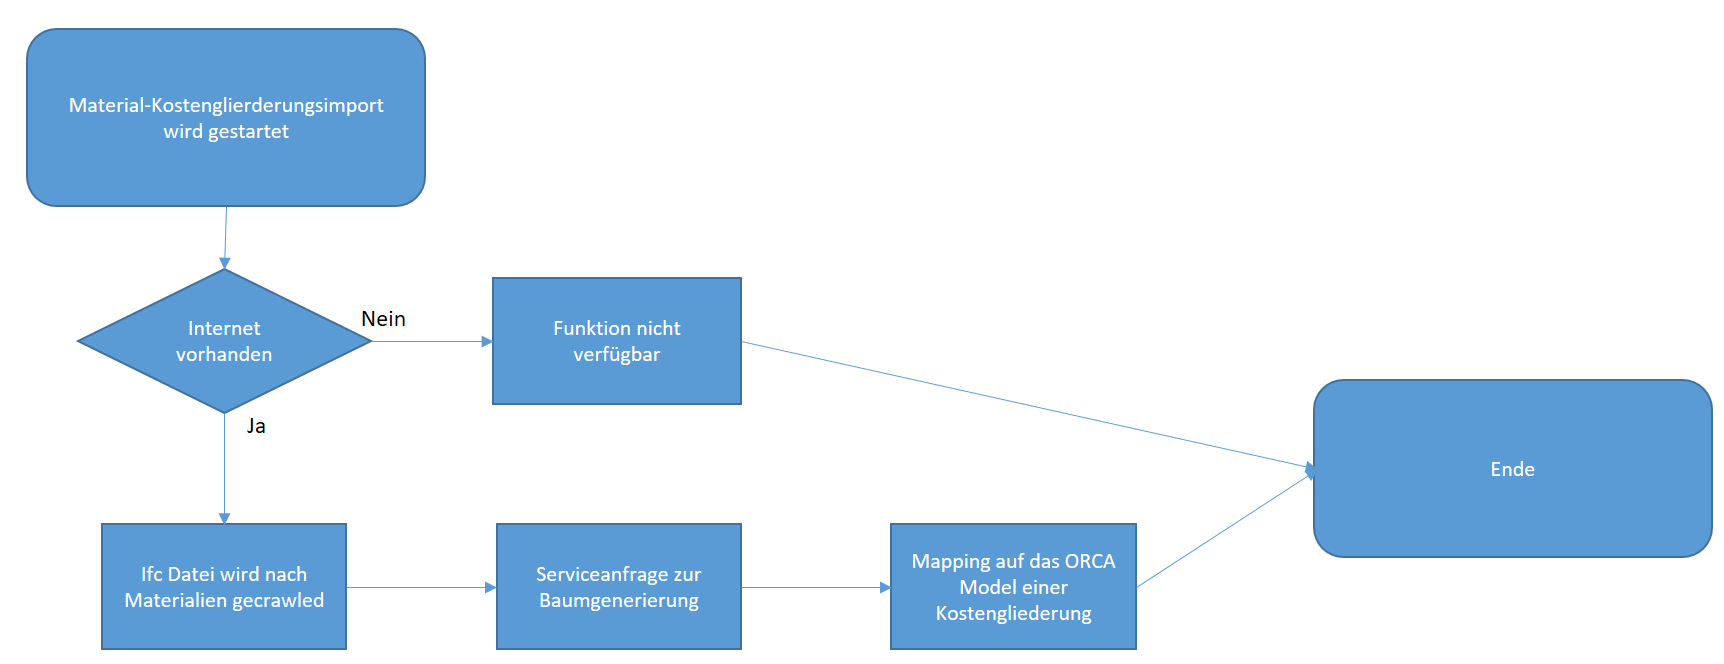
\includegraphics[width=1\linewidth]{function-import}
	\caption[Import]{Flussdiagramm Import der Material-Kostengliederung}
	\label{fig:func-import}
\end{figure}

\begin{figure}[h]
	\centering
	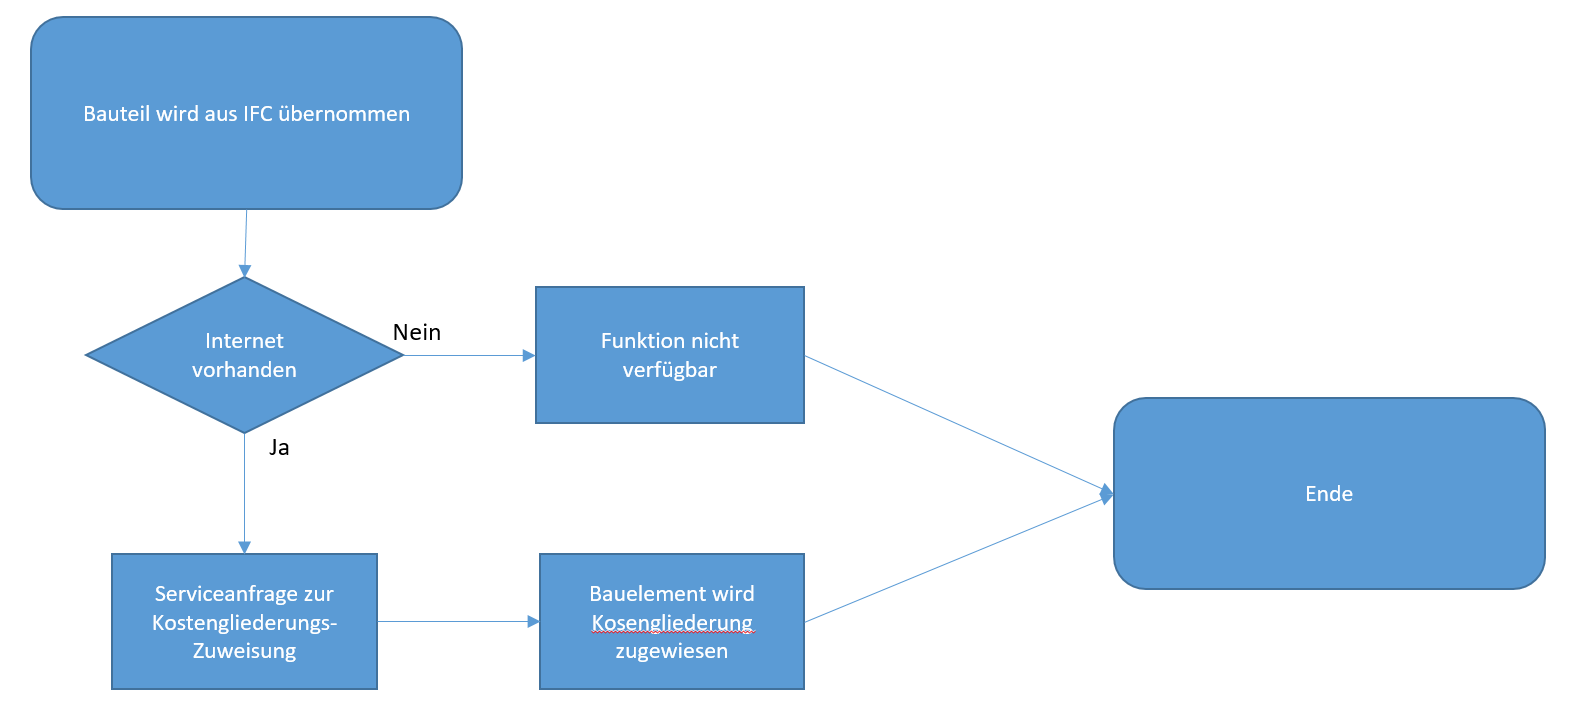
\includegraphics[width=1\linewidth]{function-takeover}
	\caption[Takeover]{Flussdiagramm Übernahme von Mengen aus dem \ac{ifc} Manager}
	\label{fig:func-takeover}
\end{figure}

\begin{figure}[h]
	\centering
	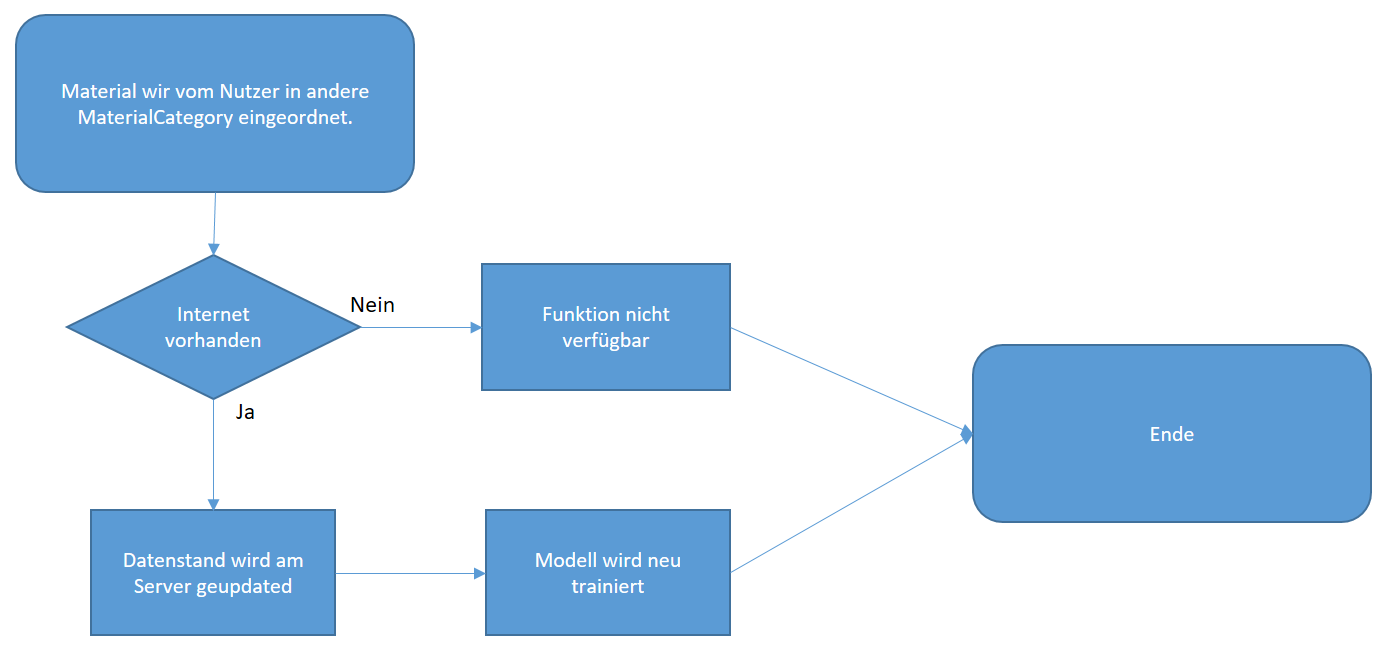
\includegraphics[width=1\linewidth]{function-rating}
	\caption[Rating]{Flussdiagramm Bewertung des Kostengliederungs-Import}
	\label{fig:func-rating}
\end{figure}

\begin{sidewaysfigure}[h]
	\centering
	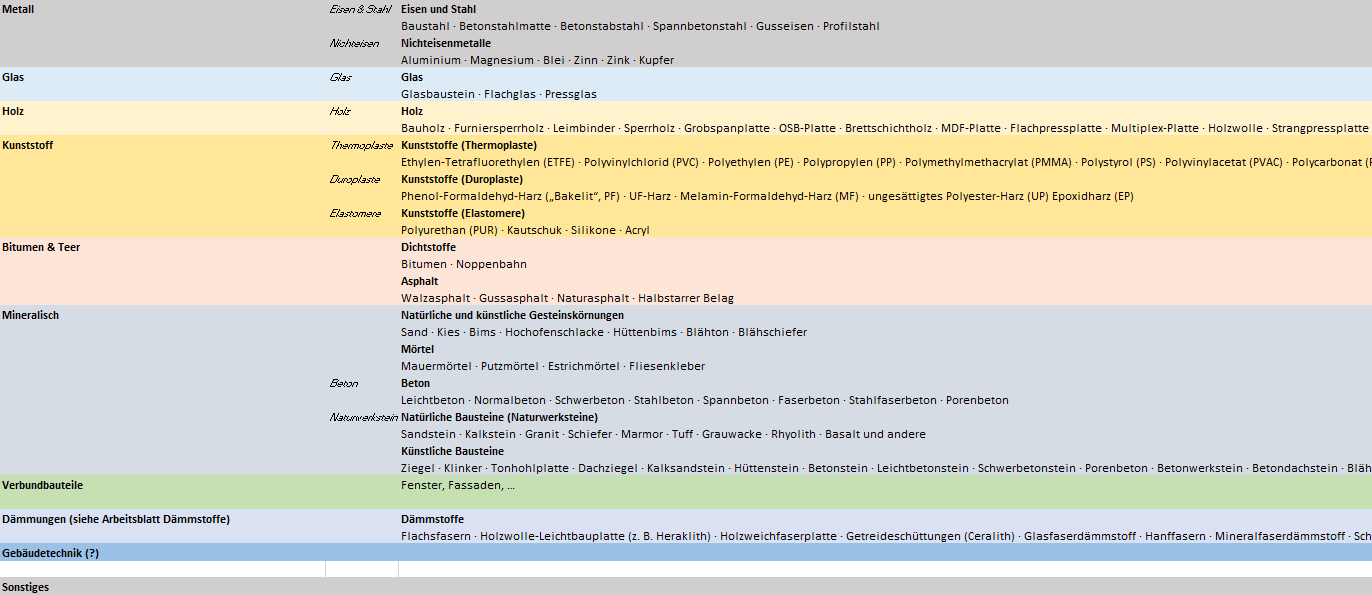
\includegraphics[width=\textheight]{material-categories}
	\caption[MaterialCategories]{}
	\label{fig:material-categories}
\end{sidewaysfigure}